%!TEX root = ../thesis.tex

% https://akhiluk.medium.com/on-why-salvor-hardin-is-simply-the-best-74948711e136
\begin{savequote}[70mm]
	To succeed, planning alone is insufficient.\\One must improvise as well.
	\qauthor{Isaac Asimov, Foundation series}
\end{savequote}

%	Writing a related work section
%	https://www.seas.upenn.edu/~cse400/CSE400_2008_2009/related_work.pdf
%	Your review should: 
%	• Summarize existing research, products and systems 
%	• Talk about trends in the field 
%	• Discuss research themes that emerged from your review 
%	• Place your work in the context of cited work 
%	• Explain why the proposed project is better than or different from what already exists

\chapter{Related work}\label{chapter:related_work}

	% https://ieeexplore.ieee.org/document/7968828
	Internet  of  Things  is  one  of  the  hottest  topics  in 
	both  industry  and  academia  of  the  communication  engineering 
	world.
	% TODO citare capitolo 2 dove parlo delle aziende di iot
	% TODO parlare della rete mesh
	On  the  other  hand,  wireless  mesh  networks,  a  network 
	topology that has been discuss for decades that haven’t been put 
	into use in large scale, can make a difference when it comes to the 
	network  in  the  IoT  world  today.

	This chapter anticipates the one where the actual project is described and shows some related projects from which the open mesh has drawn inspiration.
	
	A  wireless  mesh  network  (WMN)  is  a  communications 
	network made up of radio nodes organized in a mesh topology 
	instead of star topology
	\cite{wms}
	
	At first challenges and solutions are presented for these WMS
	
	Below are also presented some of the projects which have been made at various levels from amateurial projects, to research and to the ones already available on the market.
	
	\section{Challenges and solutions of wireless mesh networks}
		
		As explained in chap3, a mesh network is ... riprendere cosa è stato detto in chap3
		
		% https://beyondroot.com/blog/a-comprehensive-guide-to-mesh-network-in-iot-an-experts-take/
		% Where IoT Mesh Network Can be Usednostro
		
		With new technologies, wireless mesh networking has reached a point of maturity and become ideal for IoT app developers. Besides, the elevation of connected homes and industry support on open-source resources has made mesh truly accessible and low-cost. They are also regarded as much more viable and real choice for commercial as well as industrial IoT apps. At the same time, it can render extra services in a system where extending a two-node connection is limited.
		
		There are various applications for this network topology
		Smart Cities: extending radio signals through campus grounds, business parks, parking garages, and other outdoor facilities
		Healthcare Equipment: monitoring and locating medical equipment. It can also serve as a backup for medical devices that always require to stay online. Thus, if one node crashes and loses connectivity, another node can step in to maintain the connection.
		Smart Home: You can track and manage temperature across your home using a wireless mesh network. You can also capture live data and adjust settings automatically by setting up one powered gateway, sensors, and mesh-enabled nodes in each room.
		Farming: Mesh networking is the best way to track sun exposure and water levels across the crops and fields. Additionally, you can create a cellular-connected IoT platform by building a mesh network across a whole acreage with the help of an IoT app development company.
	
		Before choosing a mesh network topology it is important to evaluate
		Installation
		Device Management
		Support
	
		% https://ieeexplore.ieee.org/document/7968828
		% TODO citare + ref chap2
		Classic network topologies / architectures, which are not designed for iot networks, might not suffice the needs
		
		These computer 
		networks  are  not  designed  for  low-powered  devices  such  as 
		remote  sensors  even  these  IoT  devices  are  considered  to  be 
		mini  computers
		
		The  single  point  of  failure  nature  of  these  
		Network makes the entire system extremely vulnerable when it 
		comes to disasters or even difficult environment as the sensors 
		may need to be deployed into some hardly reachable locations.
		Besides,  the  capacity  of  the  central  hub/router  of  the  network  
		can  also  limit  the  coverage  of  the  service  provided  by  IoT  
		devices,  and the range is  also constrained by  the  same  factors.
	
		% https://galileodiscovery.unipd.it/discovery/fulldisplay?docid=alma9938985032206046&context=L&vid=39UPD_INST:VU1&lang=it&search_scope=catalogo_no_external&adaptor=Local%20Search%20Engine&tab=Everything&query=any,contains,Wireless%20Mesh%20Networks&offset=0
		Energy management is an important factor as well, since the connected devices might not have a constant source of power
		
		energy efficient transmission techniques and protocols must be developed in order to optimally use the batteries on the devices
		
		% https://galileodiscovery.unipd.it/discovery/fulldisplay?docid=alma9938986439606046&context=L&vid=39UPD_INST:VU1&lang=it&search_scope=catalogo_no_external&adaptor=Local%20Search%20Engine&tab=Everything&query=any,contains,Wireless%20Mesh%20Networks&offset=0
		
		That is why there is a particular network topology, Low Power Wireless Area Network, which is focused on the interconnection of these devices
	
		% https://ieeexplore.ieee.org/document/4068249
		
		Solutions to optimize the networks are being implemented both via hardware and software
		
		Spiegare le varie soluzioni hw, dalle board migliori, e le soluzioni sw, implementazione dell'intelligenza artificiale, fare alcuni esempi e magari citare progetti presentati successivamente.
	
	\section{Overview of wireless mesh networks}
	
		% https://www.sciencedirect.com/topics/computer-science/wireless-multihop-network
		A WMS is a particular multihop network where data is sent from a node to another until it reaches its destination
		
		An example of a multi hop wireless mesh network is VANET
		VANET is a particular case of wireless multihop network, which has the constraint of fast topology changes due to the high node mobility With the increasing number of vehicles equipped with computing technologies and wireless communication devices, intervehicle communication is becoming a promising field of research, standardization, and development. VANETs enable a wide range of applications, such as prevention of collisions, safety, blind crossing, dynamic route scheduling, real-time traffic condition monitoring, etc.
		\cite{BADIS2015653}
		
		% TODO Aggiungere citazione
		% https://www.microsoft.com/en-us/research/project/self-organizing-wireless-mesh-networks/#overview
		Microsoft has also tried to apply mesh networking to normal internet household use, however, given the improvements in telecom infrastructures and the advancement of fiber optics and internet via cable, the project has been abandoned.
		This shows how each network topology is better suited for particular scenarios.
		
		Compared to the example of microsoft's project, a vanet is more suited for a wms since the data transfered among cars is less than the one transfered among houses.
		
		\noindent
		\begin{minipage}{0.52\textwidth}% adapt widths of minipages to your needs
			\begin{figure}[H]
				\centering
				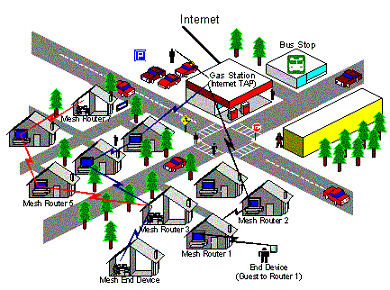
\includegraphics[width=\textwidth]{resources/img/chap4/wms_microsoft}
				\caption[Self Organizing Wireless Mesh Networks]{Self Organizing Wireless Mesh Networks\cite{BADIS2015653}}
				\label{img:wms_microsoft}
			\end{figure}
		\end{minipage}%
		\hfill%
		\begin{minipage}{0.48\textwidth}\raggedright
			\begin{figure}[H]
				\centering
				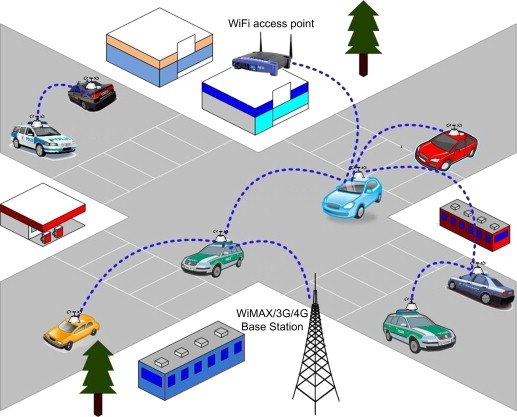
\includegraphics[width=\textwidth]{resources/img/chap4/vanet}
				\caption[An example of a VANET]{An example of a VANET\cite{BADIS2015653}}
				\label{img:vanet}
			\end{figure}
		\end{minipage}
		
	
		% https://haltian.com/resource/top-four-mesh-networks/
	
		% https://www.intechopen.com/chapters/13038
	
		% https://beyondroot.com/blog/a-comprehensive-guide-to-mesh-network-in-iot-an-experts-take/
	
		\subsection{Advantages of WMS}
		
		\subsection{Disasvantages of WMS}
	
	\section{Algorithms for Wireless Mesh networks}
	
						
	
	\section{Projects}
		
		\subsection{Open source projects}
		

			% https://www.hackster.io/scottpowell69/lora-mesh-chat-5267d9
			\subsubsection{LoRa Mesh Chat}
			
				A simple add-on for mobile phones to enable SMS-like messaging in a group when outside cell coverage, or in disaster scenarios.
				
				\noindent
				\begin{minipage}{0.48\textwidth}% adapt widths of minipages to your needs
					\begin{figure}[H]
						\centering
						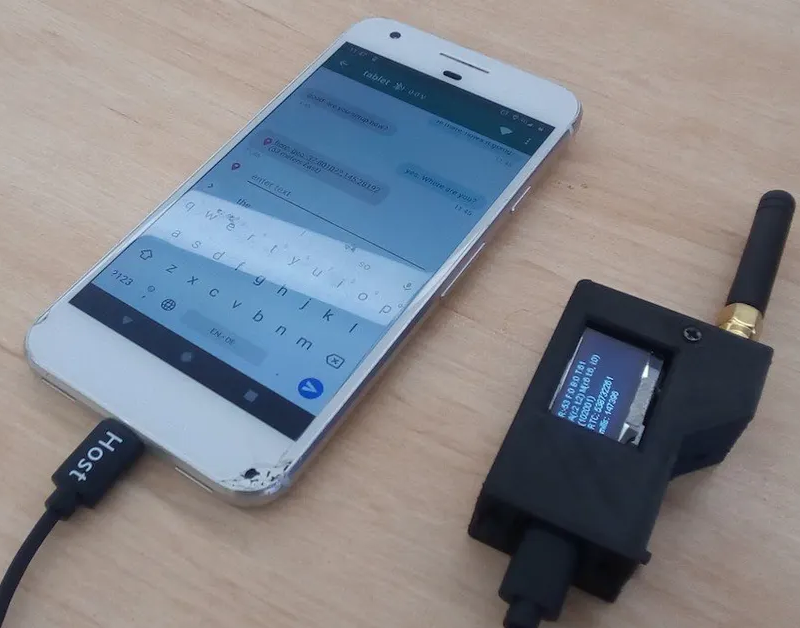
\includegraphics[width=\textwidth]{resources/img/chap4/lora-mesh-chat-5267d9}
						\caption[Self Organizing Wireless Mesh Networks]{Self Organizing Wireless Mesh Networks\cite{BADIS2015653}}
						\label{img:wms_microsoft}
					\end{figure}
				\end{minipage}%
				\hfill%
				\begin{minipage}{0.5\textwidth}\raggedright
					This is a fairly simple add-on for mobile phones to enable SMS-like messaging in a group when outside cell coverage, or in disaster scenarios. It utilises Semtech LoRa radios, for low-power/long-range communications. There are a lot of hardware options, and I am still trying different devices and manufacturers, but for now this tutorial will show how to assemble and set up one of the following boards:
					
					This board is quite nice in that it includes a nice OLED screen and Bluetooth radio. Unfortunately, the LoRa radio is not as good as the Feather, and only seems to get about half the range.
				\end{minipage}
			
				
				\subsection{Meshtastic}		
	
					% https://meshtastic.org/
					% https://github.com/meshtastic
					% https://www.hackster.io/punkgeek/meshtastic-a-hiking-skiing-gps-mesh-communicator-84f999
						
					Meshtastic is an open-source hiking, pilot, skiing, Signal app-extending GPS mesh communicator.
					
					Meshtastic is a project that lets you use inexpensive (\$30 ish) GPS radios as an extensible, super long battery life mesh GPS communicator. These radios are great for hiking, skiing, paragliding - essentially any hobby where you don’t have reliable internet access. Each member of your private mesh can always see the location and distance of all other members and any text messages sent to your group chat.
					
					The radios automatically create a mesh to forward packets as needed, so everyone in the group can receive messages from even the furthest member. The radios will optionally work with your phone, but no phone is required.Our device code is here, our optional Android app is here.
					
					Prebuilt binaries are included on the github sites, but it is quite easy to build from source. Instructions are included in the README. No soldering is required, essentially - buy a \$30 radio and go. We'd love to have your help extending the project - it has been super fun to work on.
		
		\subsection{Research projects}
		
			% https://www.springerprofessional.de/en/research-on-using-the-aodv-protocol-for-a-lora-mesh-network/18715992
			
			% BLUETOOTH
			% https://www.ericsson.com/en/reports-and-papers/white-papers/bluetooth-mesh-networking
			
			% https://ieeexplore.ieee.org/document/8071545
			
			\subsubsection{LoRaCTP}
			
				% https://ieeexplore.ieee.org/document/9394317
			
				\begin{figure}[H]
					\centering
					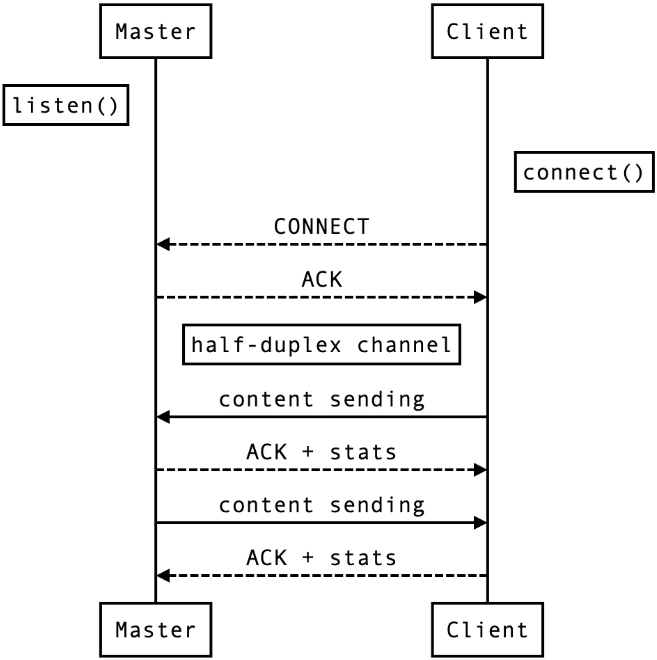
\includegraphics[width=.5\textwidth]{resources/img/loractp_flow}
					\caption{Flow of the establishment and interchange of data in LoRaCTP}
				\end{figure}
		
		\subsection{Market solutions}
		
			% https://www.kickstarter.com/projects/sonnet/sonnet-decentralized-mobile-communication
			% https://www.indiegogo.com/projects/sonnet-game-changer-for-wilderness-communications#/
			\subsubsection{Sonnet}
		
				\noindent
				\begin{minipage}{0.48\textwidth}% adapt widths of minipages to your needs
					\begin{figure}[H]
						\centering
						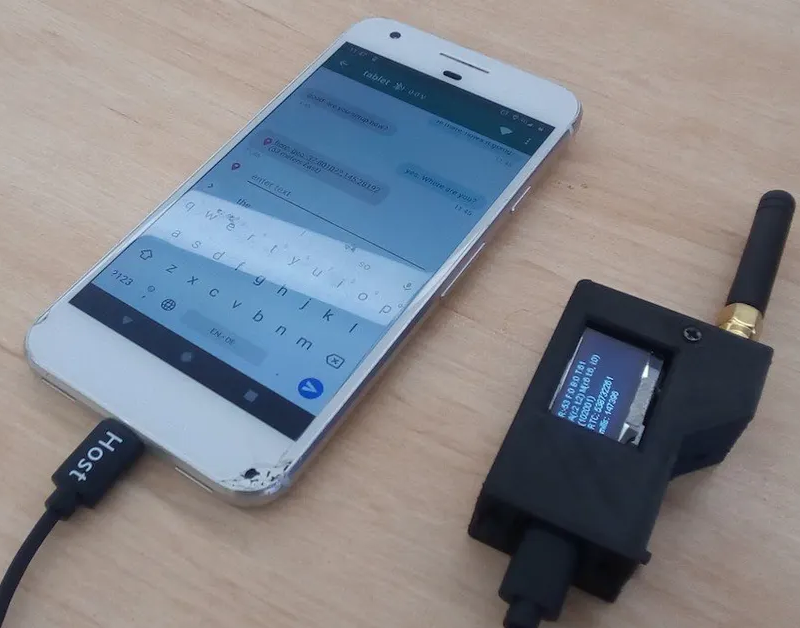
\includegraphics[width=\textwidth]{resources/img/chap4/lora-mesh-chat-5267d9}
						\caption[Self Organizing Wireless Mesh Networks]{Self Organizing Wireless Mesh Networks\cite{BADIS2015653}}
						\label{img:wms_microsoft}
					\end{figure}
				\end{minipage}%
				\hfill%
				\begin{minipage}{0.5\textwidth}\raggedright

Sonnet is the world's most advanced off-grid mobile mesh network.

The device wirelessly connects to your smartphone, etc to let you send text, voice message, images, data, files and share GPS locations to any other Sonnet users up to several kilometers away with no cell tower, no satellite, and no subscription of any kind.

Sonnet brings the long-range wireless communication of the walkie-talkie to the smartphone. It connects to your smartphone via Wi-Fi, and it will relay any data sent from your phone to other Sonnet devices via the long-range radio wave. This completely removes your smartphones’ dependency on cellular grid and other network infrastructure, and allows it to be used even when you have no cellular connectivity or internet access.

Sonnet's mesh network dramatically increases the effective range beyond point-to-point range by relaying data through other deices. With Sonnet, data can be relayed up to 16 times to achieve a maximum range of 80 km (50 miles)!
				\end{minipage}
		

			\subsubsection{goTenna}
				
%				https://gotennamesh.com/products/mesh?utm_source=internal-link&utm_medium=menu&utm_campaign=gotenna.com
						
			% https://gotenna.com/
			
			
			% https://www.project-owl.com/
			% https://www.reddit.com/r/RTLSDR/comments/bzian5/ltt_showcases_new_lora_mesh_network_devices/
		
			Pycom itself has an available mesh network that connects lora devices, compared to the one proposed in this paper thought
			% https://docs.pycom.io/pymesh/
			
			% Mesh network in other areas
			% https://www.vmware.com/products/tanzu-service-mesh.html